\documentclass{article}

% Language setting
% Replace `english' with e.g. `spanish' to change the document language
\usepackage[english]{babel}

% Set page size and margins
% Replace `letterpaper' with `a4paper' for UK/EU standard size
\usepackage[letterpaper,top=2cm,bottom=2cm,left=3cm,right=3cm,marginparwidth=1.75cm]{geometry}

% Useful packages
\usepackage{amsmath}
\usepackage{graphicx}
\usepackage{float}
\usepackage[colorlinks=true, allcolors=blue]{hyperref}

\title{Astronomy \& Astroplysics Assignment 1}
\author{Sujoy Karmakar}

\begin{document}
\maketitle

All codes are uploaded to the GitHub repository. The link is:


\verb|https://github.com/Sujoy7471/A-A2_Assignments/tree/main/Assignment%201|

%------------------------------------------------------------------------------------------------------------------

\section{Question 1:}
In this problem, the form of the radiative transfer equation that we have to use is,

\begin{equation}
-\hat{r}\left(\vec{\nabla}_{\rm rad} I \right)
= -\alpha_\nu(r,\theta) I(r,\theta) + j_\nu(r,\theta)
\end{equation}

or,

\begin{equation}
-\frac{dI}{dr} + \alpha_\nu(r,\theta) I(r,\theta) = j_\nu(r,\theta)
\end{equation}

\subsection{a:}
 Given,

\begin{equation}
\alpha_\nu(r,\theta) = \alpha_{\nu 0}\, r \cos^2\theta
\end{equation}

\begin{equation}
j_\nu(r,\theta) = j_{\nu 0}\frac{\cos^2\theta}{r}
\end{equation}

Where $\alpha_{\nu 0}$ and $j_{\nu 0}$ are constants.

Putting in (2),

\begin{equation}
-\frac{dI}{dr} + \alpha_{\nu 0} r \cos^2\theta\, I
= j_{\nu 0}\frac{\cos^2\theta}{r}
\end{equation}

or,

\begin{equation}
\frac{d}{dr}
\left(
I e^{-\frac{\alpha_{\nu 0}\cos^2\theta\, r^2}{2}}
\right)
=
-\frac{j_{\nu 0}\cos^2\theta}{r}
e^{-\frac{\alpha_{\nu 0}\cos^2\theta\, r^2}{2}}
\end{equation}

or,

\begin{equation}
\int_{I_0}^{I}
d\left(
I e^{-\frac{\alpha_{\nu 0}\cos^2\theta\, r^2}{2}}
\right)
=
-\int_{R_0}^{r}
\frac{j_{\nu 0}\cos^2\theta}{r_1}
e^{-\frac{\alpha_{\nu 0}\cos^2\theta\, r_1^2}{2}} dr_1
\end{equation}

or,

\begin{equation}
I(r,\theta)e^{-\frac{\alpha_{\nu 0}\cos^2\theta\, r^2}{2}}
-
I_0 e^{-\frac{\alpha_{\nu 0}\cos^2\theta\, R_0^2}{2}}
=
- j_{\nu 0}\cos^2\theta
\int_{R_0}^{r}
e^{-\frac{\alpha_{\nu 0}\cos^2\theta\, r_1^2}{2}}
\frac{dr_1}{r_1}
\end{equation}

Now, for $r = 0$,

\begin{equation}
I(0,\theta)
=
I_0 e^{-\frac{\alpha_{\nu 0}\cos^2\theta}{2}R_0^2}
+
j_{\nu 0}\cos^2\theta
\int_0^{R_0}
\frac{e^{-\frac{\alpha_{\nu 0}\cos^2\theta\, r_1^2}{2}}}{r_1} dr_1
\end{equation}

This can't be solved analytically. So, we use python. The solution is shown in the plot "Figure 1". Code : Q1.ipynb

\begin{figure}
\centering
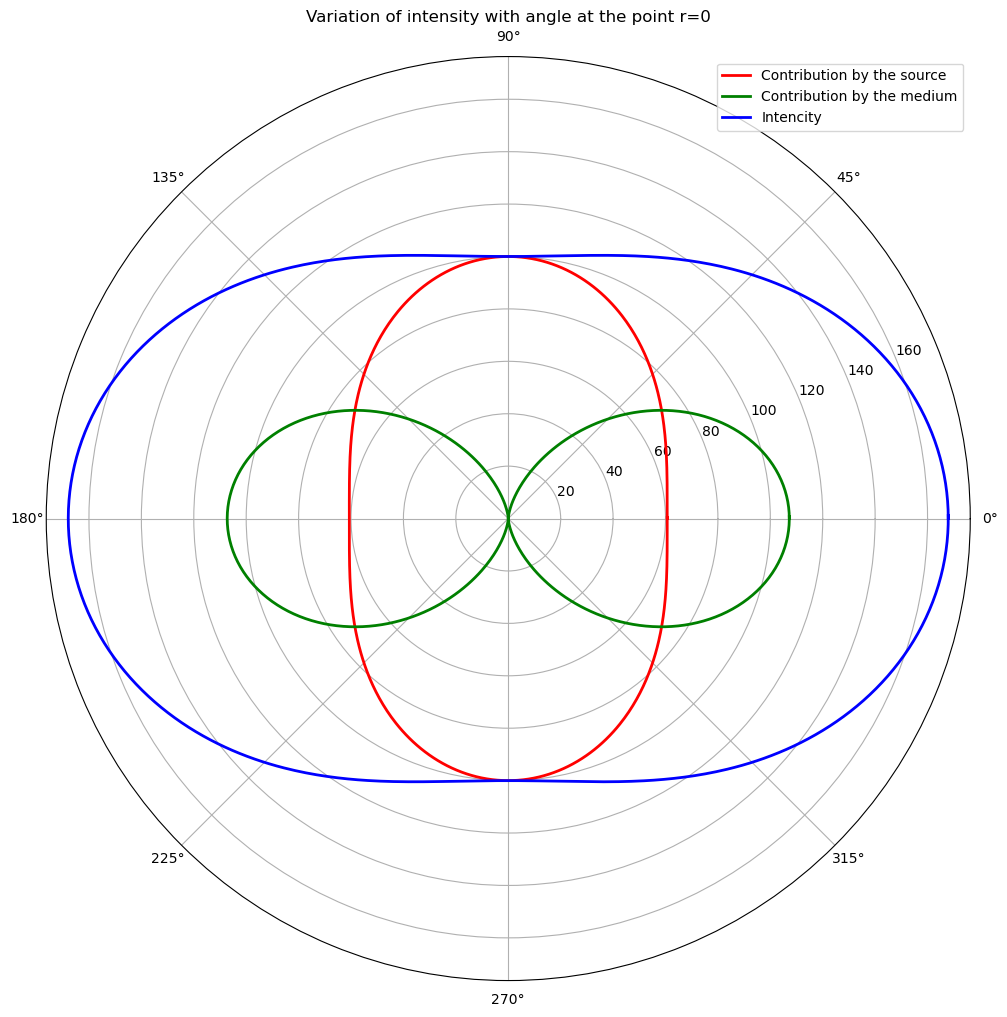
\includegraphics[width=0.5\linewidth]{Images/output_1a.png}
\caption{\label{fig:1a} Intensity Variation at r = 0}
\end{figure}

\subsection{b:}
 Given,


\begin{equation}
\alpha_\nu(r,\theta) = \alpha_{\nu 0}\, r e^{-r/R_0}
\end{equation}

\begin{equation}
j_\nu(r,\theta) = j_{\nu 0}\cos\theta \sin\theta
\end{equation}

Where $\alpha_{\nu 0}$ and $j_{\nu 0}$ are constants.

Putting in (2),

\begin{equation}
-\frac{dI}{dr} + \alpha_{\nu 0} r e^{-r/R_0} I
= j_{\nu 0}\cos\theta \sin\theta
\end{equation}

or,

\begin{equation}
\frac{dI}{dr} - \alpha_{\nu 0} r e^{-r/R_0} I
= - j_{\nu 0}\cos\theta \sin\theta
\end{equation}

Multiplying by the integrating factor,

\begin{equation}
\mu(r)=e^{-\int \alpha_{\nu 0} r e^{-r/R_0} dr}
\end{equation}

we obtain

\begin{equation}
\frac{d}{dr}
\left(
I e^{-\int \alpha_{\nu 0} r e^{-r/R_0} dr}
\right)
=
- j_{\nu 0}\cos\theta \sin\theta
e^{-\int \alpha_{\nu 0} r e^{-r/R_0} dr}
\end{equation}

Integrating,

\begin{equation}
I(r,\theta)e^{-\int \alpha_{\nu 0} r e^{-r/R_0} dr}
-
I_0 e^{-\int_{0}^{R_0} \alpha_{\nu 0} r e^{-r/R_0} dr}
=
- j_{\nu 0}\cos\theta \sin\theta
\int_{R_0}^{r}
e^{-\int \alpha_{\nu 0} r e^{-r/R_0} dr} dr
\end{equation}

Now, for $r=0$,

\begin{equation}
I(0,\theta)
=
I_0 e^{-\int_{0}^{R_0} \alpha_{\nu 0} r e^{-r/R_0} dr}
+
j_{\nu 0}\cos\theta \sin\theta
\int_0^{R_0}
e^{-\int \alpha_{\nu 0} r e^{-r/R_0} dr} dr
\end{equation}

This also cannot be solved analytically. So, we use python. The solution is shown in the plot "Figure 2". Code : Q1.ipynb

\begin{figure}
\centering
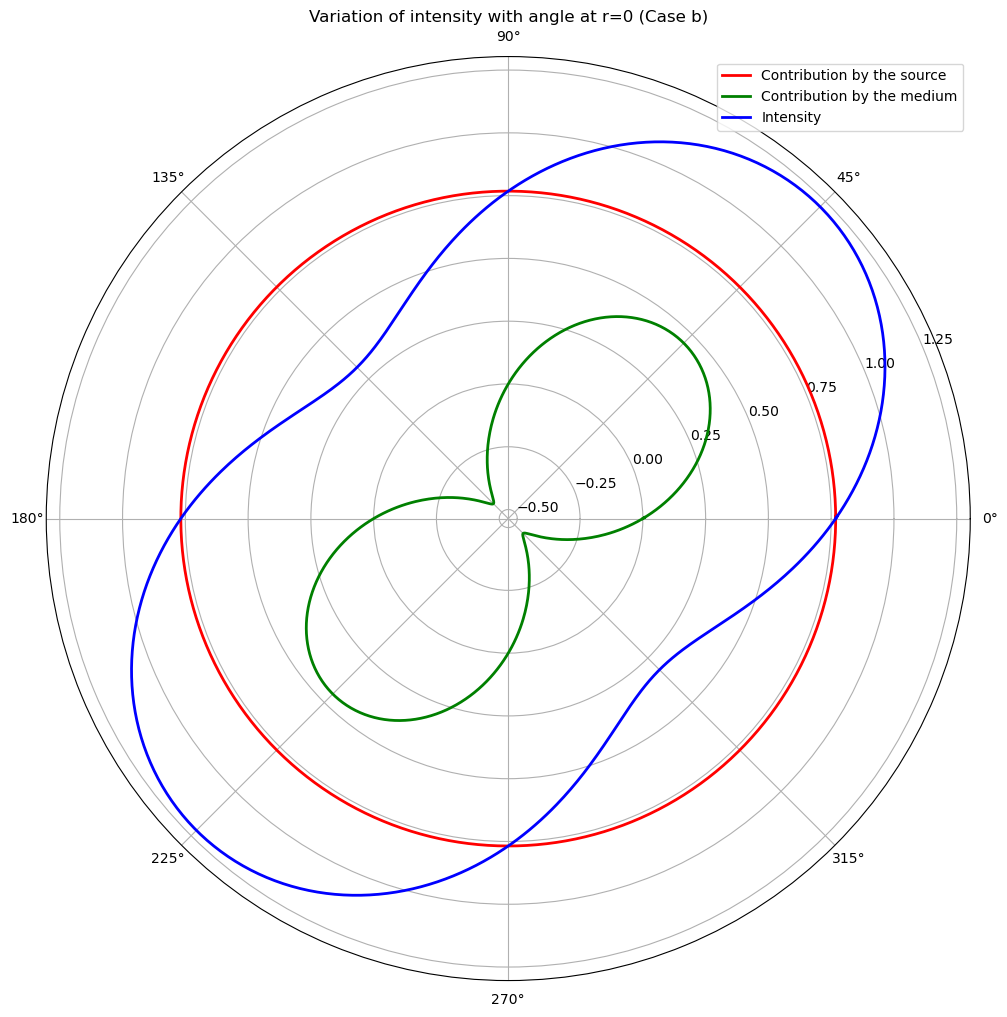
\includegraphics[width=0.5\linewidth]{Images/output_1b.png}
\caption{\label{fig:1a} Intensity Variation at r = 0}
\end{figure}



\subsection{c:}
 Given,


\begin{equation}
\alpha_\nu(r,\theta) = \alpha_{\nu 0}\, r \ln\left(\frac{r}{R_0}\right)
\end{equation}

\begin{equation}
j_\nu(r,\theta) = j_{\nu 0} r
\end{equation}

Where $\alpha_{\nu 0}$ and $j_{\nu 0}$ are constants.

Putting in (2),

\begin{equation}
-\frac{dI}{dr} + \alpha_{\nu 0} r \ln\left(\frac{r}{R_0}\right) I
= j_{\nu 0} r
\end{equation}

or,

\begin{equation}
\frac{dI}{dr} - \alpha_{\nu 0} r \ln\left(\frac{r}{R_0}\right) I
= - j_{\nu 0} r
\end{equation}

Multiplying by the integrating factor,

\begin{equation}
\mu(r)=e^{-\int \alpha_{\nu 0} r \ln\left(\frac{r}{R_0}\right) dr}
\end{equation}

we obtain

\begin{equation}
\frac{d}{dr}
\left(
I e^{-\int \alpha_{\nu 0} r \ln\left(\frac{r}{R_0}\right) dr}
\right)
=
- j_{\nu 0} r
e^{-\int \alpha_{\nu 0} r \ln\left(\frac{r}{R_0}\right) dr}
\end{equation}

Integrating,

\begin{equation}
I(r,\theta)e^{-\int \alpha_{\nu 0} r \ln\left(\frac{r}{R_0}\right) dr}
-
I_0 e^{-\int_{0}^{R_0} \alpha_{\nu 0} r \ln\left(\frac{r}{R_0}\right) dr}
=
- j_{\nu 0}
\int_{R_0}^{r}
r_1 e^{-\int \alpha_{\nu 0} r_1 \ln\left(\frac{r_1}{R_0}\right) dr_1}
dr_1
\end{equation}

Now, for $r=0$,

\begin{equation}
I(0,\theta)
=
I_0 e^{-\int_{0}^{R_0} \alpha_{\nu 0} r \ln\left(\frac{r}{R_0}\right) dr}
+
j_{\nu 0}
\int_0^{R_0}
r_1 e^{-\int \alpha_{\nu 0} r_1 \ln\left(\frac{r_1}{R_0}\right) dr_1}
dr_1
\end{equation}

This also cannot be solved analytically. So, we use python. The solution is shown in the plot "Figure 3". Code : Q1.ipynb

\begin{figure}
\centering
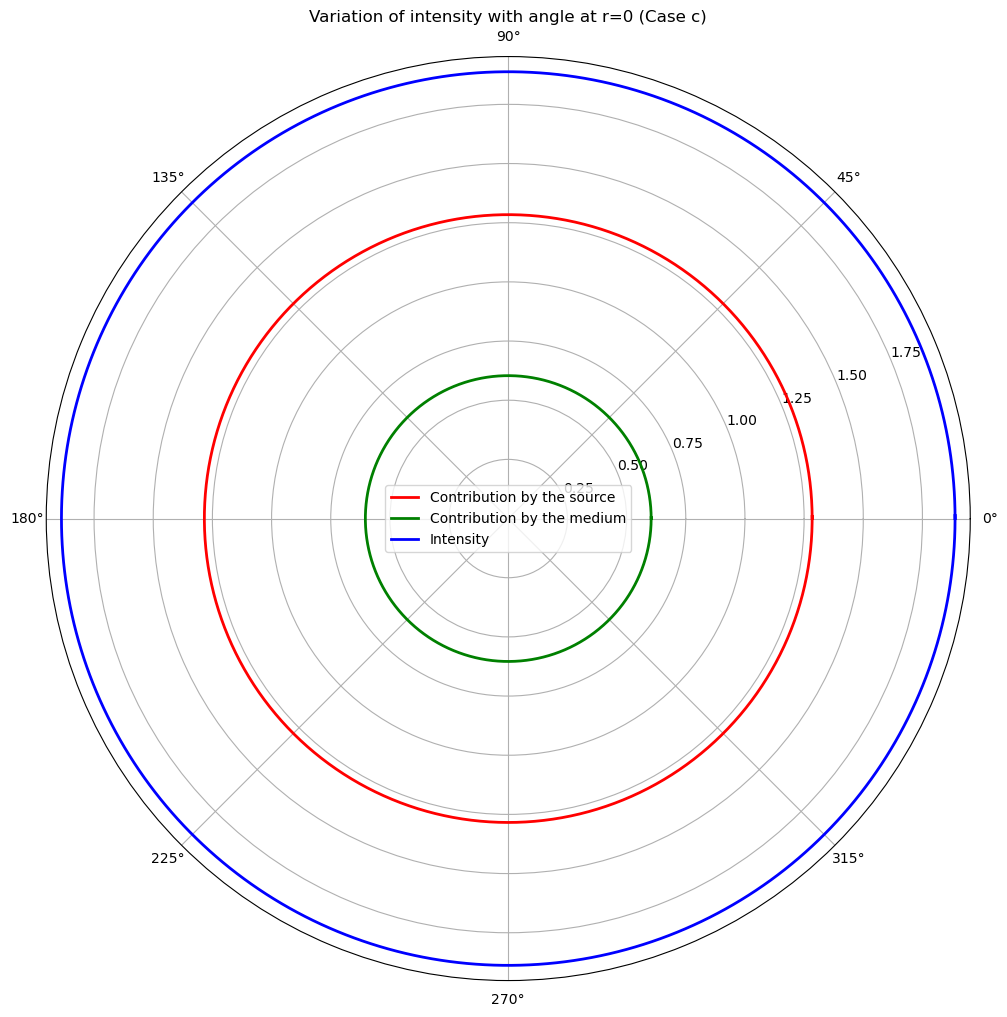
\includegraphics[width=0.5\linewidth]{Images/output_1c.png}
\caption{\label{fig:1a} Intensity Variation at r = 0}
\end{figure}





%----------------------------------------------------------------------------------------------------------------
\section{Question 2:}

We know, optical depth in this case,

\begin{equation}
\tau_\nu(r,\theta)=\int_r^{R_0}\alpha_\nu(r',\theta)dr'
\end{equation}

The code for this question is, "Q2.ipynb"
\subsection{i)}

\subsubsection{a)}

From question 1.a,

\begin{equation}
\alpha_\nu=\alpha_{\nu 0} r\cos^2\theta
\end{equation}

So,

\begin{equation}
\tau_\nu(r,\theta)=\int_r^{R_0}\alpha_{\nu 0} r' \cos^2\theta \,dr'
\end{equation}

\begin{equation}
\tau_\nu(r,\theta)=\frac{\alpha_{\nu 0}\cos^2\theta}{2}(R_0^2-r^2)
\end{equation}

Then,

\begin{equation}
\tau_\nu(r)=\int_0^{2\pi}\tau_\nu(r,\theta)d\theta
\end{equation}

\begin{equation}
\boxed{
\tau_\nu(r)=\frac{\pi\alpha_{\nu 0}}{2}(R_0^2-r^2)
}
\end{equation}

This is the required expression.

---

\subsubsection{b)}

From question 1.b,

\begin{equation}
\alpha_\nu=\alpha_{\nu 0} r e^{-r/R_0}
\end{equation}

So,

\begin{equation}
\tau_\nu(r,\theta)=\int_r^{R_0}\alpha_{\nu 0} r' e^{-r'/R_0}dr'
\end{equation}

Since $\alpha_\nu$ is independent of $\theta$,

\begin{equation}
\tau_\nu(r)=\int_0^{2\pi}\tau_\nu(r,\theta)d\theta
\end{equation}

\begin{equation}
\tau_\nu(r)=2\pi\alpha_{\nu 0}\int_r^{R_0} r' e^{-r'/R_0}dr'
\end{equation}

\begin{equation}
\boxed{
\tau_\nu(r)
=
2\pi\alpha_{\nu0}
\left[
R_0(r+R_0)e^{-r/R_0}
-
2R_0^2e^{-1}
\right]
}
\end{equation}

This is the required expression.

---

\subsubsection{c)}

From question 1.c,

\begin{equation}
\alpha_\nu=\alpha_{\nu 0} r\ln\left(\frac{r}{R_0}\right)
\end{equation}

So,

\begin{equation}
\tau_\nu(r,\theta)=\int_r^{R_0}\alpha_{\nu 0} r'\ln\left(\frac{r'}{R_0}\right)dr'
\end{equation}

Again $\alpha_\nu$ is independent of $\theta$.

\begin{equation}
\tau_\nu(r)=\int_0^{2\pi}\tau_\nu(r,\theta)d\theta
\end{equation}

\begin{equation}
\boxed{
\tau_\nu(r)=2\pi\alpha_{\nu 0}\int_r^{R_0} r'\ln\left(\frac{r'}{R_0}\right)dr'
}
\end{equation}

This is the required expression.

---

\begin{figure}[H]
\centering
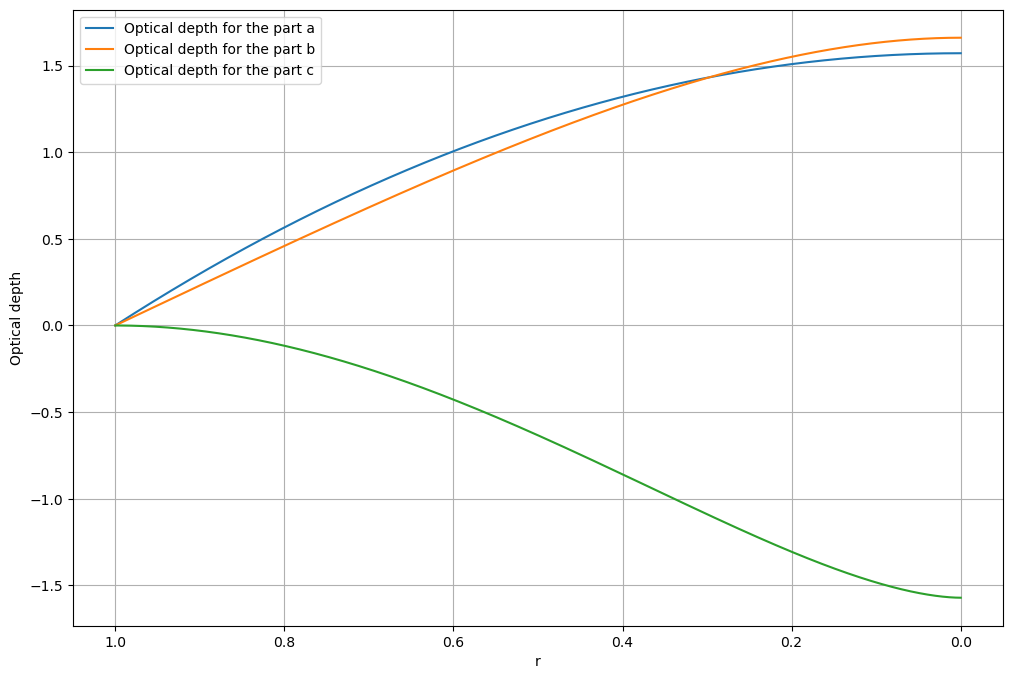
\includegraphics[width=0.5\linewidth]{Images/output_2.png}
\caption{\label{fig:2} Optical depth as radial inward distance}
\end{figure}

Here we can see in the image "Figure 4" that for the "part c", the optical depth is negative. This is actually anticipated as the given value of the absorption coefficient is negative in the range $r \in [0, R_0] $


\subsection{ii)}

\subsubsection{a)}

From equation (3),

\begin{equation}
\frac{\partial\tau}{\partial\theta}
=
-\alpha_{\nu 0}(R_0^2-r^2)\sin\theta\cos\theta
\end{equation}

At $r=\frac{R_0}{2}$,

\begin{equation}
\boxed{
\left.\frac{\partial\tau}{\partial\theta}\right|_{R_0/2}
=
-\frac{3\alpha_{\nu 0}R_0^2}{4}\sin\theta\cos\theta
}
\end{equation}

At $r=\frac{R_0}{4}$,

\begin{equation}
\boxed{
\left.\frac{\partial\tau}{\partial\theta}\right|_{R_0/4}
=
-\frac{15\alpha_{\nu 0}R_0^2}{16}\sin\theta\cos\theta
}
\end{equation}

---

\subsubsection{b)}

Since $\alpha_\nu$ is independent of $\theta$, the optical depth is also independent of $\theta$.

\begin{equation}
\frac{\partial\tau}{\partial\theta}=0
\end{equation}

Therefore,

\begin{equation}
\boxed{
\left.\frac{\partial\tau}{\partial\theta}\right|_{R_0/2}=0
}
\end{equation}

\begin{equation}
\boxed{
\left.\frac{\partial\tau}{\partial\theta}\right|_{R_0/4}=0
}
\end{equation}

---

\subsubsection{c)}

Similarly, $\alpha_\nu$ is independent of $\theta$.

\begin{equation}
\frac{\partial\tau}{\partial\theta}=0
\end{equation}

Thus,

\begin{equation}
\boxed{
\left.\frac{\partial\tau}{\partial\theta}\right|_{R_0/2}=0
}
\end{equation}

\begin{equation}
\boxed{
\left.\frac{\partial\tau}{\partial\theta}\right|_{R_0/4}=0
}
\end{equation}



%------------------------------------------------------------------------------------------
\section{Question 3:}

Here given that the medium undergoes both absorption and scattering. The radiative transfer equation then becomes

\begin{equation}
-\frac{dI_\nu}{dr}=-(\alpha_\nu+\sigma_\nu)I_\nu+(\alpha_\nu+\sigma_\nu) S_\nu
\end{equation}

where $\sigma_\nu$ is the scattering coefficient. The negative sign is because we are moving from r = $R_0$ to r = 0.

Given that the scattering coefficient is $20\%$ of the absorption coefficient,

\begin{equation}
\sigma_\nu = 0.2\,\alpha_\nu
\end{equation}

So the total extinction coefficient becomes

\begin{equation}
\chi_\nu = \alpha_\nu + \sigma_\nu
\end{equation}

\begin{equation}
\chi_\nu = 1.2\,\alpha_\nu
\end{equation}

The optical depth is therefore

\begin{equation}
\tau_\nu(r,\theta)=\int_r^{R_0}\chi_\nu(r',\theta)dr'
\end{equation}

\subsection{a}


From Question 1.a,

\begin{equation}
\alpha_\nu(r,\theta)=\alpha_{\nu0} r\cos^2\theta
\end{equation}

So,

\begin{equation}
\chi_\nu(r,\theta)=1.2\alpha_{\nu0} r\cos^2\theta
\end{equation}

Putting in (50),

\begin{equation}
-\frac{dI}{dr}+1.2\alpha_{\nu0} r\cos^2\theta I
=
1.2\alpha_{\nu0} r\cos^2\theta S_\nu
\end{equation}

or,

\begin{equation}
\frac{dI}{dr}-1.2\alpha_{\nu0} r\cos^2\theta I
=
-1.2\alpha_{\nu0} r\cos^2\theta S_\nu
\end{equation}

Multiplying by the integrating factor,

\begin{equation}
\mu(r)=e^{-\int1.2\alpha_{\nu0} r\cos^2\theta dr}
\end{equation}

\begin{equation}
\mu(r)=e^{-0.6\alpha_{\nu0} r^2\cos^2\theta}
\end{equation}

we obtain

\begin{equation}
\frac{d}{dr}
\left(
I e^{-0.6\alpha_{\nu0} r^2\cos^2\theta}
\right)
=
-1.2\alpha_{\nu0} r\cos^2\theta S_\nu
e^{-0.6\alpha_{\nu0} r^2\cos^2\theta}
\end{equation}

Integrating,

\begin{equation}
I(r,\theta)e^{-0.6\alpha_{\nu0} r^2\cos^2\theta}
-
I_0 e^{-0.6\alpha_{\nu0} R_0^2\cos^2\theta}
=
-
\int_{R_0}^{r}
1.2\alpha_{\nu0} r'\cos^2\theta S_\nu
e^{-0.6\alpha_{\nu0} r'^2\cos^2\theta}dr'
\end{equation}

Now for $r=0$,

\begin{equation}
\boxed{
I(0,\theta)
=
I_0 e^{-0.6\alpha_{\nu0} R_0^2\cos^2\theta}
+
\int_0^{R_0}
1.2\alpha_{\nu0} r'\cos^2\theta S_\nu
e^{-0.6\alpha_{\nu0} r'^2\cos^2\theta}dr'
}
\end{equation}

This is the required intensity value for the case where source function is non zero.
This cannot be solved analytically.\\

Now for the case when $S_\nu=0$,

\begin{equation}
\boxed{
I(0,\theta)=I_0 e^{-0.6\alpha_{\nu0} R_0^2\cos^2\theta}
}
\end{equation}

The optical depth in both of the cases

\begin{equation}
\tau_\nu(r,\theta)=\int_r^{R_0}1.2\alpha_{\nu0} r'\cos^2\theta dr'
\end{equation}

\begin{equation}
\boxed{
\tau_\nu(0,\theta)=0.6\alpha_{\nu0}R_0^2\cos^2\theta
}
\end{equation}

\subsection{b}

From Question 1.b,

\begin{equation}
\alpha_\nu(r)=\alpha_{\nu0} r e^{-r/R_0}
\end{equation}

So,

\begin{equation}
\chi_\nu(r)=1.2\alpha_{\nu0} r e^{-r/R_0}
\end{equation}

Putting in (50),

\begin{equation}
-\frac{dI}{dr}+1.2\alpha_{\nu0} r e^{-r/R_0} I
=
1.2\alpha_{\nu0} r e^{-r/R_0} S_\nu
\end{equation}

or,

\begin{equation}
\frac{dI}{dr}-1.2\alpha_{\nu0} r e^{-r/R_0} I
=
-1.2\alpha_{\nu0} r e^{-r/R_0} S_\nu
\end{equation}

Multiplying by the integrating factor,

\begin{equation}
\mu(r)=e^{-\int1.2\alpha_{\nu0} r e^{-r/R_0} dr}
\end{equation}

we obtain

\begin{equation}
\frac{d}{dr}
\left(
I e^{-\int1.2\alpha_{\nu0} r e^{-r/R_0} dr}
\right)
=
-1.2\alpha_{\nu0} r e^{-r/R_0} S_\nu
e^{-\int1.2\alpha_{\nu0} r e^{-r/R_0} dr}
\end{equation}

Integrating,

\begin{equation}
I(r)e^{-\int1.2\alpha_{\nu0} r e^{-r/R_0} dr}
-
I_0 e^{-\int_{0}^{R_0}1.2\alpha_{\nu0} r e^{-r/R_0} dr}
=
-
\int_{R_0}^{r}
1.2\alpha_{\nu0} r' e^{-r'/R_0} S_\nu
e^{-\int1.2\alpha_{\nu0} r' e^{-r'/R_0} dr'} dr'
\end{equation}

Now for $r=0$,

\begin{equation}
\boxed{
I(0)
=
I_0 e^{-\int_{0}^{R_0}1.2\alpha_{\nu0} r e^{-r/R_0} dr}
+
\int_0^{R_0}
1.2\alpha_{\nu0} r' e^{-r'/R_0} S_\nu
e^{-\int1.2\alpha_{\nu0} r' e^{-r'/R_0} dr'} dr'
}
\end{equation}

This is the required intensity value for the case where source function is non zero.
This cannot be solved complete analytically.\\

Now for the case when $S_\nu=0$,

\begin{equation}
\boxed{
I(0)=I_0 e^{-\int_{0}^{R_0}1.2\alpha_{\nu0} r e^{-r/R_0} dr}
}
\end{equation}

The optical depth in both of the cases

\begin{equation}
\tau_\nu(r)=\int_r^{R_0}1.2\alpha_{\nu0} r' e^{-r'/R_0} dr'
\end{equation}

or,

\begin{equation}
\boxed{
\tau_\nu(0)=1.2\alpha_{\nu0}R_0^2(1-2e^{-1})
}
\end{equation}



\subsection{c}

From Question 1.c,

\begin{equation}
\alpha_\nu(r)=\alpha_{\nu0} r\ln\left(\frac{r}{R_0}\right)
\end{equation}

So,

\begin{equation}
\chi_\nu(r)=1.2\alpha_{\nu0} r\ln\left(\frac{r}{R_0}\right)
\end{equation}

Putting in (50),

\begin{equation}
-\frac{dI}{dr}+1.2\alpha_{\nu0} r\ln\left(\frac{r}{R_0}\right) I
=
1.2\alpha_{\nu0} r\ln\left(\frac{r}{R_0}\right) S_\nu
\end{equation}

or,

\begin{equation}
\frac{dI}{dr}-1.2\alpha_{\nu0} r\ln\left(\frac{r}{R_0}\right) I
=
-1.2\alpha_{\nu0} r\ln\left(\frac{r}{R_0}\right) S_\nu
\end{equation}

Multiplying by the integrating factor,

\begin{equation}
\mu(r)=e^{-\int1.2\alpha_{\nu0} r\ln\left(\frac{r}{R_0}\right) dr}
\end{equation}

we obtain

\begin{equation}
\frac{d}{dr}
\left(
I e^{-\int1.2\alpha_{\nu0} r\ln\left(\frac{r}{R_0}\right) dr}
\right)
=
-1.2\alpha_{\nu0} r\ln\left(\frac{r}{R_0}\right) S_\nu
e^{-\int1.2\alpha_{\nu0} r\ln\left(\frac{r}{R_0}\right) dr}
\end{equation}

Integrating,

\begin{equation}
I(r)e^{-\int1.2\alpha_{\nu0} r\ln\left(\frac{r}{R_0}\right) dr}
-
I_0 e^{-\int_{0}^{R_0}1.2\alpha_{\nu0} r\ln\left(\frac{r}{R_0}\right) dr}
=
-
\int_{R_0}^{r}
1.2\alpha_{\nu0} r'\ln\left(\frac{r'}{R_0}\right) S_\nu
e^{-\int1.2\alpha_{\nu0} r'\ln\left(\frac{r'}{R_0}\right) dr'} dr'
\end{equation}

Now for $r=0$,

\begin{equation}
\boxed{
I(0)
=
I_0 e^{-\int_{0}^{R_0}1.2\alpha_{\nu0} r\ln\left(\frac{r}{R_0}\right) dr}
+
\int_0^{R_0}
1.2\alpha_{\nu0} r'\ln\left(\frac{r'}{R_0}\right) S_\nu
e^{-\int1.2\alpha_{\nu0} r'\ln\left(\frac{r'}{R_0}\right) dr'} dr'
}
\end{equation}

This is the required intensity value for the case where source function is non zero.
This cannot be solved analytically.\\

Now for the case when $S_\nu=0$,

\begin{equation}
\boxed{
I(0)=I_0 e^{-\int_{0}^{R_0}1.2\alpha_{\nu0} r\ln\left(\frac{r}{R_0}\right) dr}
}
\end{equation}

The optical depth in both of the cases

\begin{equation}
\tau_\nu(r)=\int_r^{R_0}1.2\alpha_{\nu0} r'\ln\left(\frac{r'}{R_0}\right) dr'
\end{equation}

or, 

\begin{equation}
\boxed{
\tau_\nu(0)=-0.3\alpha_{\nu0}R_0^2
}
\end{equation}

[Yeah this is negative. This is because of the form of the absorption coefficient.]





%-------------------------------------------------------------------------------------
\section{Question 4:}

In the Rayleigh-Jeans regime the intensity is proportional to the brightness temperature,

\begin{equation}
I_\nu = \frac{2k\nu^2}{c^2}T_b
\end{equation}

So the radiative transfer equation can be written in terms of brightness temperature as

\begin{equation}
\frac{dT_b}{d\tau}=-(T_b-T)
\end{equation}

where $T$ is the physical temperature of the medium.

Solving this differential equation,

\begin{equation}
T_b = T_b(0)e^{-\tau} + T(1-e^{-\tau})
\end{equation}

Given that the temperature of the material is

\begin{equation}
T = 1000\ K
\end{equation}

we obtain

\begin{equation}
T_b = T_b(0)e^{-\tau} + 1000(1-e^{-\tau})
\end{equation}

\subsection{i) Initial brightness temperature = 100 K}

Putting $T_b(0)=100$,

\begin{equation}
T_b = 100 e^{-\tau} + 1000(1-e^{-\tau})
\end{equation}

\begin{equation}
\boxed{
T_b = 1000 - 900e^{-\tau}
}
\end{equation}

Now we already have for part a,
\begin{equation}
\tau_\nu(0,\theta)=0.6\alpha_{\nu0}R_0^2\cos^2\theta
\end{equation}


For part b,
\begin{equation}
\tau_\nu(0)=1.2\alpha_{\nu0}R_0^2(1-2e^{-1})
\end{equation}

For part c,
\begin{equation}
\tau_\nu(0)=-0.3\alpha_{\nu0}R_0^2
\end{equation}

Substituting these values of $\tau$ into the expressions above gives the brightness temperature for each case.

\subsection{ii) Initial brightness temperature = $10^4$ K}

Putting $T_b(0)=10^4$,

\begin{equation}
T_b = 10^4 e^{-\tau} + 1000(1-e^{-\tau})
\end{equation}

\begin{equation}
\boxed{
T_b = 1000 + 9000e^{-\tau}
}
\end{equation}
 

Now we already have for part a,
\begin{equation}
\tau_\nu(0,\theta)=0.6\alpha_{\nu0}R_0^2\cos^2\theta
\end{equation}


For part b,
\begin{equation}
\tau_\nu(0)=1.2\alpha_{\nu0}R_0^2(1-2e^{-1})
\end{equation}

For part c,
\begin{equation}
\tau_\nu(0)=-0.3\alpha_{\nu0}R_0^2
\end{equation}

Substituting these values of $\tau$ into the expressions above gives the brightness temperature for each case.




%--------------------------------------------------------------------------------------------------------------------------
\section{Question 5:}

The total radiated power of an accelerated charged particle is given by the Larmor formula

\begin{equation}
P=\frac{2q^2a^2}{3c^3}
\end{equation}

In this problem the particle has charge $4q$, so

\begin{equation}
P=\frac{2(4q)^2a^2}{3c^3}
\end{equation}

\begin{equation}
P=\frac{32q^2a^2}{3c^3}
\end{equation}

\subsection{a}

The trajectory is given by

\begin{equation}
x(t)=R_0\cos(\omega t)
\end{equation}

\begin{equation}
y(t)=R\sin(\omega t)
\end{equation}

\begin{equation}
z(t)=R
\end{equation}

The velocity components are

(As nothing has been mentioned about $R_0$ and R, so for simplicity in calculation, I'm taking them as constants)

\begin{equation}
\dot{x}=-R_0\omega\sin(\omega t)
\end{equation}

\begin{equation}
\dot{y}=R\omega\cos(\omega t)
\end{equation}

\begin{equation}
\dot{z}=0
\end{equation}

The acceleration components are

\begin{equation}
\ddot{x}=-R_0\omega^2\cos(\omega t)
\end{equation}

\begin{equation}
\ddot{y}=-R\omega^2\sin(\omega t)
\end{equation}

\begin{equation}
\ddot{z}=0
\end{equation}

So the magnitude of the acceleration is

\begin{equation}
a^2=\ddot{x}^2+\ddot{y}^2
\end{equation}

\begin{equation}
a^2=
R_0^2\omega^4\cos^2(\omega t)
+
R^2\omega^4\sin^2(\omega t)
\end{equation}

\begin{equation}
a^2=\omega^4
\left(
R_0^2\cos^2(\omega t)+R^2\sin^2(\omega t)
\right)
\end{equation}

Putting this in the Larmor formula

\begin{equation}
\boxed{
P(t)=
\frac{32q^2}{3c^3}
\omega^4
\left(
R_0^2\cos^2(\omega t)+R^2\sin^2(\omega t)
\right)
}
\end{equation}

Taking the time average and using

\begin{equation}
\langle \cos^2(\omega t) \rangle =
\langle \sin^2(\omega t) \rangle = \frac12
\end{equation}

we obtain

\begin{equation}
\boxed{
\langle P \rangle =
\frac{16q^2\omega^4}{3c^3}(R_0^2+R^2)
}
\end{equation}

\subsection{b}

The trajectory is given by

\begin{equation}
x(t)=x_0\sinh(v_0 t)
\end{equation}

\begin{equation}
y(t)=y_0\sinh(v_0 t)
\end{equation}

The velocity components are

\begin{equation}
\dot{x}=x_0 v_0\cosh(v_0 t)
\end{equation}

\begin{equation}
\dot{y}=y_0 v_0\cosh(v_0 t)
\end{equation}

The acceleration components are

\begin{equation}
\ddot{x}=x_0 v_0^2\sinh(v_0 t)
\end{equation}

\begin{equation}
\ddot{y}=y_0 v_0^2\sinh(v_0 t)
\end{equation}

So the magnitude of acceleration becomes

\begin{equation}
a^2=\ddot{x}^2+\ddot{y}^2
\end{equation}

\begin{equation}
a^2=v_0^4\sinh^2(v_0 t)(x_0^2+y_0^2)
\end{equation}

Putting this in the Larmor formula

\begin{equation}
P(t)=
\frac{32q^2}{3c^3}
v_0^4\sinh^2(v_0 t)
(x_0^2+y_0^2)
\end{equation}

\begin{equation}
\boxed{
P(t)=
\frac{32q^2v_0^4}{3c^3}
(x_0^2+y_0^2)\sinh^2(v_0 t)
}
\end{equation}





%--------------------------------------------------------------------------------------------------------------------------
\section{Question 6:}










We know,

\begin{equation}
\frac{1}{\alpha_R}
=
\frac{\int_0^{\infty} (\alpha_\nu+\sigma_\nu)^{-1}
\frac{\partial B_\nu}{\partial T}\,d\nu}
{\int_0^{\infty}\frac{\partial B_\nu}{\partial T}\,d\nu}
\end{equation}

Where,

\begin{equation}
B_\nu=\frac{2h\nu^3}{c^2}\frac{1}{e^{h\nu/kT}-1}
\end{equation}

So,

\begin{equation}
\frac{\partial B_\nu}{\partial T}
=
\frac{2h\nu^3}{c^2}
\frac{1}{(e^{h\nu/kT}-1)^2}
\left(\frac{h\nu}{kT^2}\right)
\end{equation}

But in the question, for all the three cases,

\begin{equation}
\alpha_\nu \neq \alpha_\nu(\nu), \qquad
\sigma_\nu \neq \sigma_\nu(\nu)
\end{equation}

So, the expression can be written as

\begin{equation}
\frac{1}{\alpha_R}
=
\frac{(\alpha_\nu+\sigma_\nu)^{-1}
\int_0^\infty \frac{\partial B_\nu}{\partial T} d\nu}
{\int_0^\infty \frac{\partial B_\nu}{\partial T} d\nu}
\end{equation}

or,

\begin{equation}
\boxed{\alpha_R=(\alpha_\nu+\sigma_\nu)}
\end{equation}

And the Rosseland approximation for the energy flux is,

\begin{equation}
F(r)=
-\frac{16\sigma T^3}{3\alpha_R}\frac{\partial T}{\partial r}
\end{equation}

But for stars,

\begin{equation}
\frac{\partial T}{\partial r}<0
\end{equation}

So,

\begin{equation}
\boxed{
F(r)=
\frac{16\sigma T^3}{3\alpha_R}
\left|\frac{\partial T}{\partial r}\right|
}
\end{equation}

\bigskip

\textbf{i) So, for the absorption coefficient}

\medskip

\textbf{a)}

When

\begin{equation}
\alpha_\nu=\alpha_0 r^2 , \qquad
\sigma_\nu=\sigma_0 r^2
\end{equation}

\begin{equation}
\boxed{\alpha_R=(\alpha_0+\sigma_0)r^2}
\end{equation}

\medskip

\textbf{b)}

When

\begin{equation}
\alpha_\nu=\alpha_0 r , \qquad
\sigma_\nu=\sigma_0 r
\end{equation}

\begin{equation}
\boxed{\alpha_R=(\alpha_0+\sigma_0)r}
\end{equation}

\medskip

\textbf{c)}

When

\begin{equation}
\alpha_\nu=\alpha_0 e^{-r/R_0} , \qquad
\sigma_\nu=\sigma_0 e^{-r/R_0}
\end{equation}

\begin{equation}
\boxed{\alpha_R=(\alpha_0+\sigma_0)e^{-r/R_0}}
\end{equation}

\bigskip

\textbf{ii) a) The Rosseland flux is,}

\begin{equation}
\boxed{
F(r)=
\frac{16\sigma T^3}
{3(\alpha_0+\sigma_0)r^2}
\left|\frac{\partial T}{\partial r}\right|
}
\end{equation}

\medskip

\textbf{b) The Rosseland flux is,}

\begin{equation}
\boxed{
F(r)=
\frac{16\sigma T^3}
{3(\alpha_0+\sigma_0)r}
\left|\frac{\partial T}{\partial r}\right|
}
\end{equation}

\medskip

\textbf{c) The Rosseland flux is,}

\begin{equation}
\boxed{
F(r)=
\frac{16\sigma T^3}
{3(\alpha_0+\sigma_0)e^{-r/R_0}}
\left|\frac{\partial T}{\partial r}\right|
}
\end{equation}

\bigskip

Here putting values, we can get required numerical answers.

\medskip

\textbf{iii)} Now the required plot is given below. The code is \textit{Q6.ipynb}.


\begin{figure}[H]
\centering
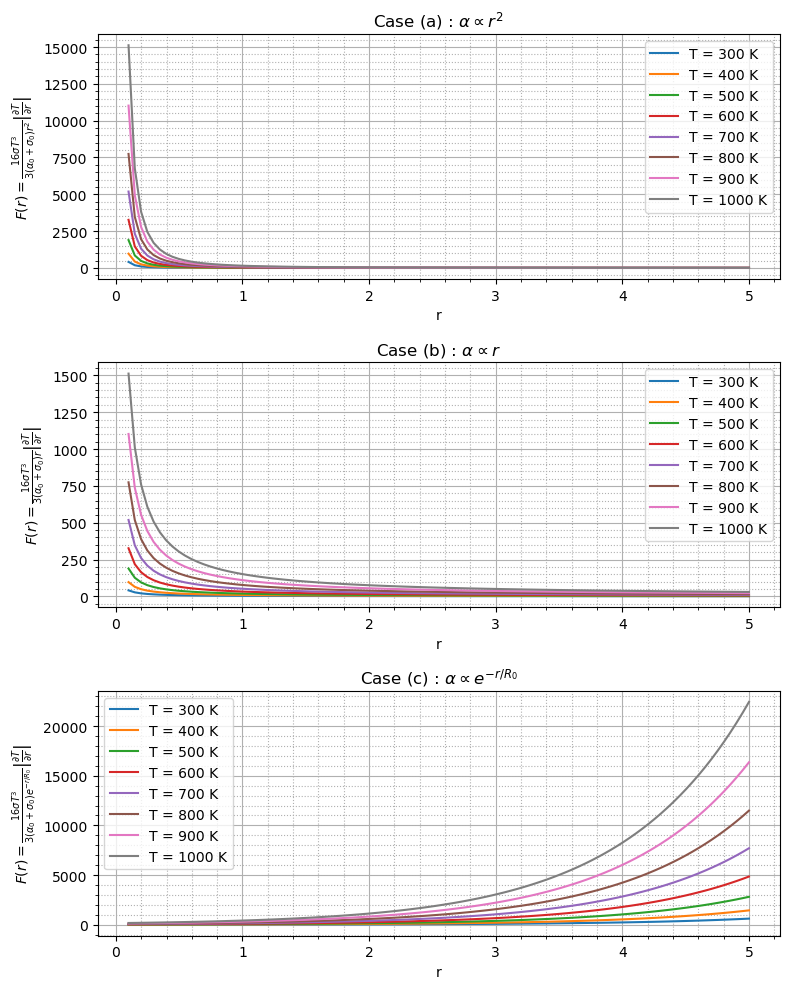
\includegraphics[width=0.6\linewidth]{Images/output_6.png}
\caption{\label{fig:6} Flux Variation with r }
\end{figure}








\end{document}

